\section{Problem 3: Derandomizing Signatures}\label{sec:problem3}

Let $\mathcal{S} = (G, S, V)$ be a secure signature scheme defined over $(\mathcal{M}, \Sigma)$, where the signing algorithm $S$ is probabilistic.
In particular, algorithm $S$ uses randomness chosen from a space $\mathcal{R}$.
We let $S(sk,m;r)$ denote the execution of algorithm $S$ with randomness $r$.
Let $F$ be a secure PRF defined over $(\mathcal{K}, \mathcal{M}, \mathcal{R})$.
Show that the following signature scheme $\mathcal{S'} = (G', S', V)$ is secure:
\begin{equation*}
    \begin{split}
        G'() &\coloneqq \{ (pk, sk) \overset{\mathcal{R}}{\longleftarrow} G(), 
            \hspace{3pt} k \overset{\mathcal{R}}{\longleftarrow} \mathcal{K}, 
            \hspace{3pt} sk' \coloneqq (sk, k), 
            \hspace{3pt} \text{output } (pk, sk') \}; \\
        S'(sk', m) &\coloneqq \{ r \longleftarrow F(k, m),
            \hspace{3pt} \sigma \longleftarrow S(sk, m; r),
            \hspace{3pt} \text{output } \sigma \}.
    \end{split}
\end{equation*}
Now the signing algorithm for $S'$ is deterministic.

\begin{center}
    \rule{5cm}{0.4pt}
\end{center}

\textbf{\textit{Proof:}}
Let us denote, for the sake of simplicity, as $S_{R}$ the \textit{randomized} signature scheme, and as $S_{DR}$ the \textit{derandomized}.
Our hypothesis is that $S_R$ is secure against a chosen message attack, as defined in the Attack Game $13.1$, and that $F$ is a secure $PRF$, as defined in Attack Game $4.2$.

We will build an attacker for the $PRF$ game, $A_{PRF}$ who acts as a challenger for Attack Game $13.1$.
The scheme is depicted in Figure \ref{fig:attack-game}

\begin{figure}[h!]
    \centering
    \begin{tikzpicture}
        % Define Variables
        \def\lR{0.75}
        \def\rR{5.35}
        \def\lDR{10.75}
        \def\rDR{15.35}
        \def\bottom{-9}

        % Overall Scheme
        \draw[thick] (0,0) -- (6,0) node[midway, anchor=south] {PRF Game $4.2$};
        \node[anchor = north west] at (0,0) (c-r) {\scriptsize Challenger};
        \draw[dotted] (\lR, -0.5) -- (\lR,\bottom);
        \node[anchor = north east, text=red] at (6,0) {\scriptsize Attacker};
        \draw[dotted] (\rR, -0.5) -- (\rR, \bottom);
        \draw[thick, dashed] (6,0) -- (6, \bottom);
        \draw[thick] (10,0) -- (16,0) node[midway, anchor=south] {Signature Game $13.1$};
        \node[anchor = north west, text=red] at (10,0) {\scriptsize Challenger};
        \node[anchor = north east, text=blue] at (16,0) {\scriptsize Attacker};
        \draw[thick, dashed] (10,0) -- (10, \bottom);
        \draw[dotted] (\lDR, -0.5) -- (\lDR, \bottom);
        \draw[dotted] (\rDR, -0.5) -- (\rDR, \bottom);

        % Start Games
        \draw[->] (\rR, -1) -- (\lR, -1) node[midway, anchor=south] {\scriptsize Start Game};
        \draw[->] (\lR, -1.75) -- (\rR, -1.75) node[midway, anchor=south] {};
        \node[anchor=west] at (\lR, -1.5) {$b \overset{\mathcal{R}}{\longleftarrow} \{0,1\}$};
        \node[anchor=north west, align=left] at (\lR, -1.75) {\tiny $f \overset{b=0}{\longleftarrow} F(k, \cdot)$, $k$ random seed, $F$ PRF \\ \tiny $f \overset{b=1}{\longleftarrow} Funs(\mathcal{X}, \mathcal{Y})$, $f$ random function};
        \node[anchor=east] at (\rR, -1.5) {$f$};
        \node[anchor=south east, color=red] at (\lDR, -2) {$(pk, sk) \overset{\mathcal{R}}{\longleftarrow} G()$};
        \draw[->,color=red] (\rR, -2) -- (\lDR, -2);
        \draw[->] (\lDR, -2.25) -- (\rDR, -2.25) node[anchor=south east, text=blue] {$pk$};

        % First Signing Query
        \draw[->] (\rDR, -2.75) -- (\lDR, -2.75) node[midway, anchor=south] {\scriptsize $Sign(m_1)$};
        \node[anchor=north east, text=blue] at (\rDR, -2.75) {$m_1$};
        \draw[->,color=red] (\lDR, -3) -- (\rR, -3) node[text=red,anchor=south west] {$m_1$};
        \draw[->] (\rR, -3.25) -- (\lR, -3.25) node[midway, anchor=south] {\scriptsize $Image(m_1)$};
        \node[anchor=south west] at (\lR, -4.25) {$y_1 \leftarrow f(m_1)$};
        \draw[->] (\lR, -4.25) -- (\rR, -4.25) node[anchor=south east] {$y_1$};
        \draw[->,color=red] (\rR, -4.5) -- (\lDR, -4.5) node[midway, anchor=south] {\scriptsize $\sigma_1 \overset{b=0}{\leftarrow} S(sk;m_1;F(k, m_1))$} node[midway, anchor=north] {\scriptsize $\sigma_1 \overset{b=1}{\leftarrow} S(sk;m_1;f(m_1))$};
        \draw[->] (\lDR, -4.75) -- (\rDR, -4.75) node[anchor=south east, text=blue] {$\sigma_1$};

        % Next Signing Queries
        \node[anchor=north east] at (\rDR, -4.75) {$\vdots$};
        \node[anchor=north east] at (\rDR, -5.25) {$\vdots$};
        \draw (\rDR, -6.25) node[anchor=north east, text=blue] {$m_{q_S}$} -- (14, -6.25);
        \draw[dashed] (14, -6.25) -- (13, -6.25);
        \draw[dashed] (14, -6.75) -- (13, -6.75);
        \draw[->] (14, -6.75) -- (\rDR, -6.75) node[anchor=north east, text=blue] {$\sigma_{q_S}$};

        % Forgery
        \draw[->, thick, color=blue] (\rDR, -7.75) -- (\lDR, -7.75) node[midway, anchor=south] {$(\sigma^*, m^*)$};
        \draw[->, thick, color=red] (\rR, -8.25) -- (\lR, -8.25) node[midway, anchor=south] {$\hat{b} \in \{0,1\}$};
        \draw[->, color=red] (\lDR, -8) -- (\rR, -8) node[midway, anchor=south, text=red, align=left] {\scriptsize $Pr(\hat{b} = 1 | b = 0) = \text{adv}(A_{DR})$ \\ \scriptsize $Pr(\hat{b} = 1 | b = 1) = \text{adv}(A_{R})$};
        

    \end{tikzpicture}
    \caption{Attack to the $PRF$ game using triggering an attacker for the Signature one. In red are the two roles that we actively play, and in black and blue two different entities respectively.\label{fig:attack-game}}
\end{figure}

Initially, the challenger in the $PRF$ game randomly chooses $b = 0,1$:
\begin{itemize}
    \item If $b = 0$: he picks $k \overset{R}{\longleftarrow} \mathcal{K}$ and $f \leftarrow F(k, \cdot)$ a PRF.
    \item If $b = 1$: he picks a random function $f$, that effectively given an input returns a random output.
\end{itemize}
Once we, the attacker in $PRF$, receive $f$, we call the generating algorithm $(pk, sk) \leftarrow G()$ and initialize the Signature Game by sending $pk$ to the attacker in the signature game.

For each signing query $Sign(m_i)$ we receive from the attacker, we forward $m_i$ to the challenger in $PRF$ and receive $f(m_i)$.
We then respond to the signing query with $\sigma_i \leftarrow S(sk, m_i; f(m_i))$.
Observe that:
\begin{itemize}
    \item If $b = 0$: $\sigma_i \leftarrow S(sk, m_i; F(k, m_i))$ for $F$ PRF and $k$ a random seed. Hence effectively playing the game for $S_{DR}$.
    \item If $b = 1$: $\sigma_i \leftarrow S(sk, m_i; r_i)$ for a random $r_i$. Hence effectively playing the game for $S_R$.
\end{itemize}

Once the attacker for $S$ has performed all of its signing queries, he will output a forgery candidate $(\sigma^*, m^*)$.
We will output $1$ in the $PRF$ game if the forgery is valid.
For $b = 0,1$, let $W_b$ be the event that we output $1$ in the PRF game given the value of $b$. Then,
\begin{equation*}
    \begin{split}
        Pr(W_0) &= Pr(A_{PRF} = 1 | b = 0) = Pr((\sigma^*, m^*) \text{ is a valid forgery} | b = 0) = \text{adv}(S_{DR}) \\
        Pr(W_1) &= Pr(A_{PRF} = 1 | b = 1) = Pr((\sigma^*, m^*) \text{ is a valid forgery} | b = 1) = \text{adv}(S_{R}) \\
    \end{split}
\end{equation*}
where the probability of breaking the signature game is also denoted as the advantage.

Lastly, in Definition 4.21, we define the advantage in the $PRF$ game as:
\begin{equation*}
    \begin{split}
        \text{adv}(PRF) &= Pr(W_0) - Pr(W_1) = \text{adv}(S_{DR}) - \text{adv}(S_R) \Leftrightarrow \\
        \text{adv}(S_{DR}) &= \text{adv}(PRF) + \text{adv}(S_R) \leq \varepsilon_{PRF} + \varepsilon_{R}
    \end{split}
\end{equation*}
where we have used that, as $F$ was $PRF$ secure by hypothesis, and so was $S$, the advantages in these games are neglegible, hence the advantage for $S_{DR}$ is also neglegible, and the signature scheme secure as we wanted to prove. \hfill $\qed$
